\begin{landscape}


\subsection{Other UML diagrams}


\subsubsection{Class diagram}

In this subsection a conceptual UML Class Diagram is shown.

\begin{figure}[H]
\begin{centering}
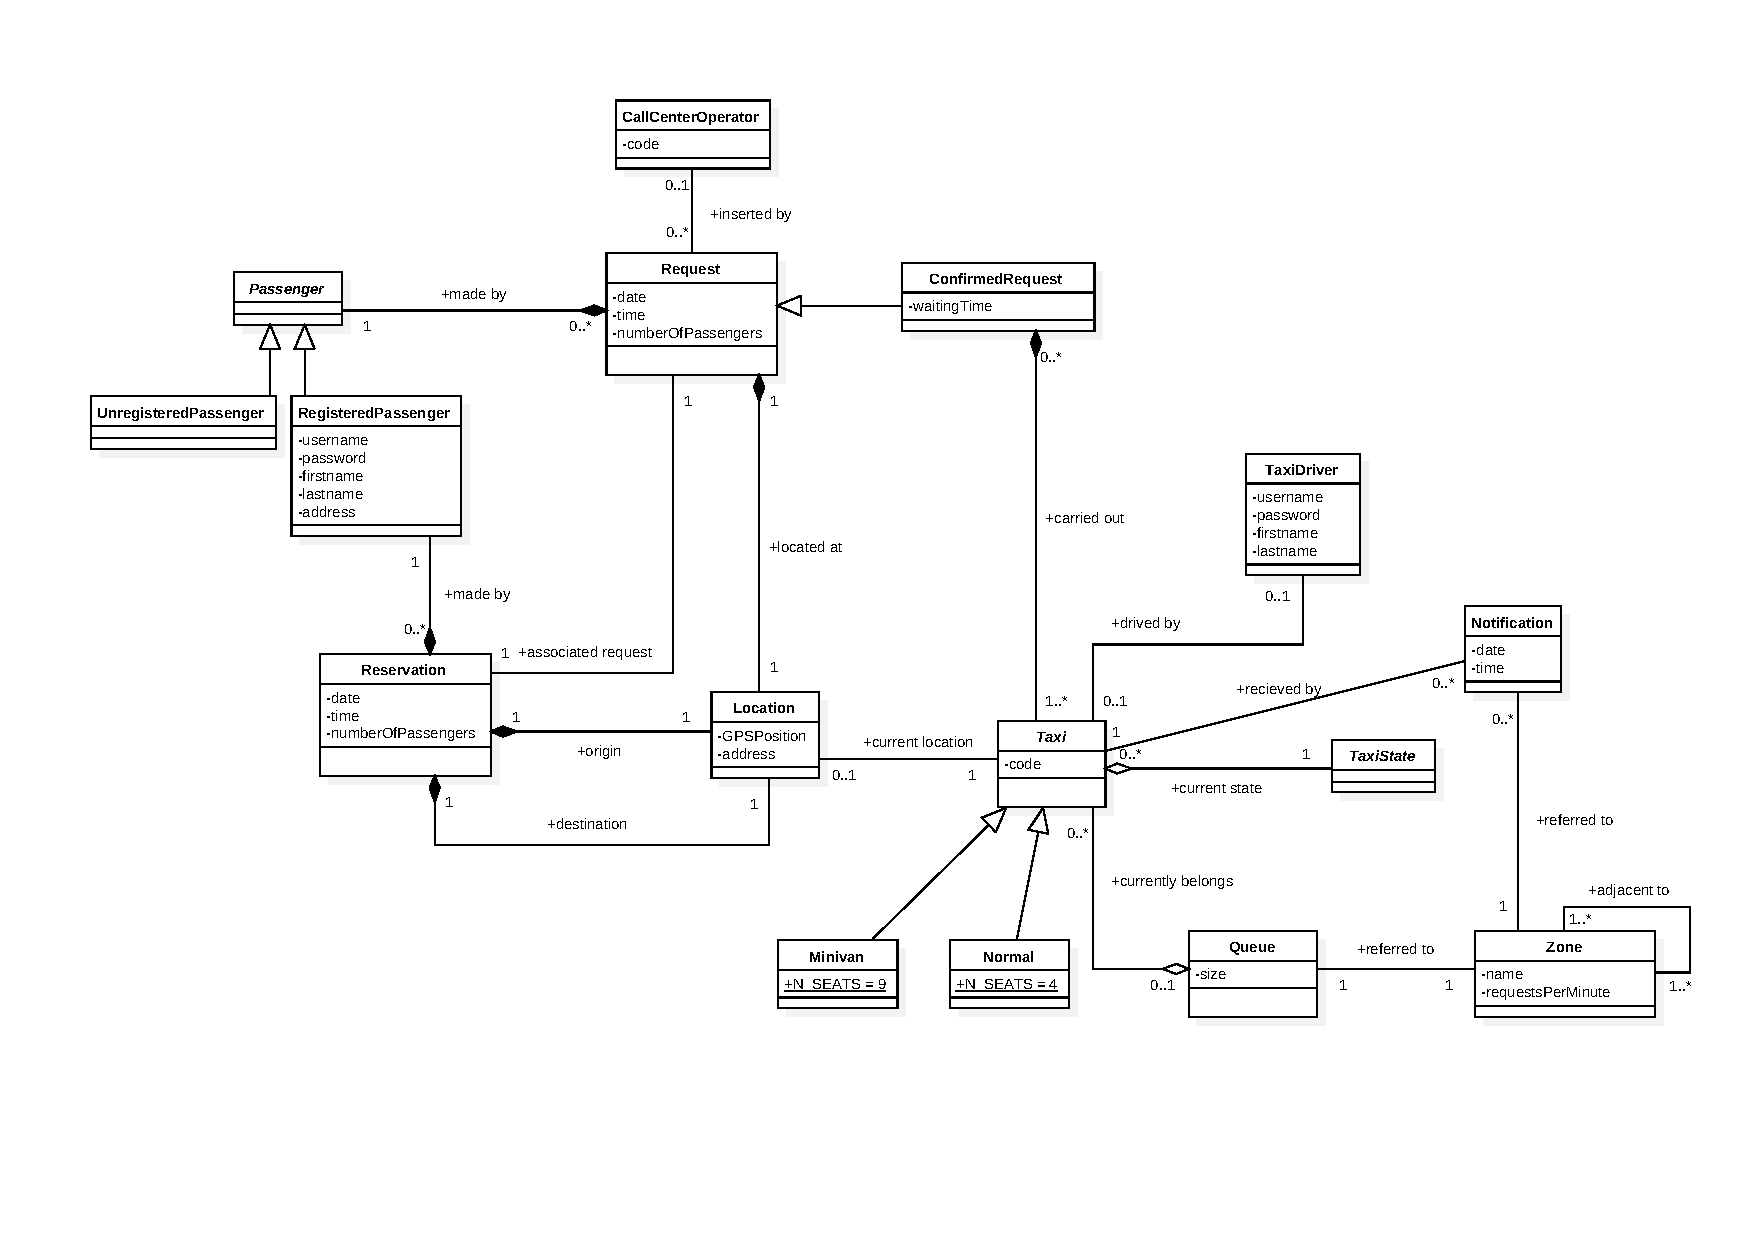
\includegraphics[bb=25bp 100bp 842bp 580bp,scale=0.65]{specific-requirements/3.6-other-uml/image/class}
\par\end{centering}

\protect\caption{UML Class Diagram}
\end{figure}


\clearpage{}


\subsubsection{State chart diagram}

In this subsection a state chart diagram is shown to make clear how
the state of a taxi changes according to the events occuring.

\begin{figure}[H]
\begin{centering}
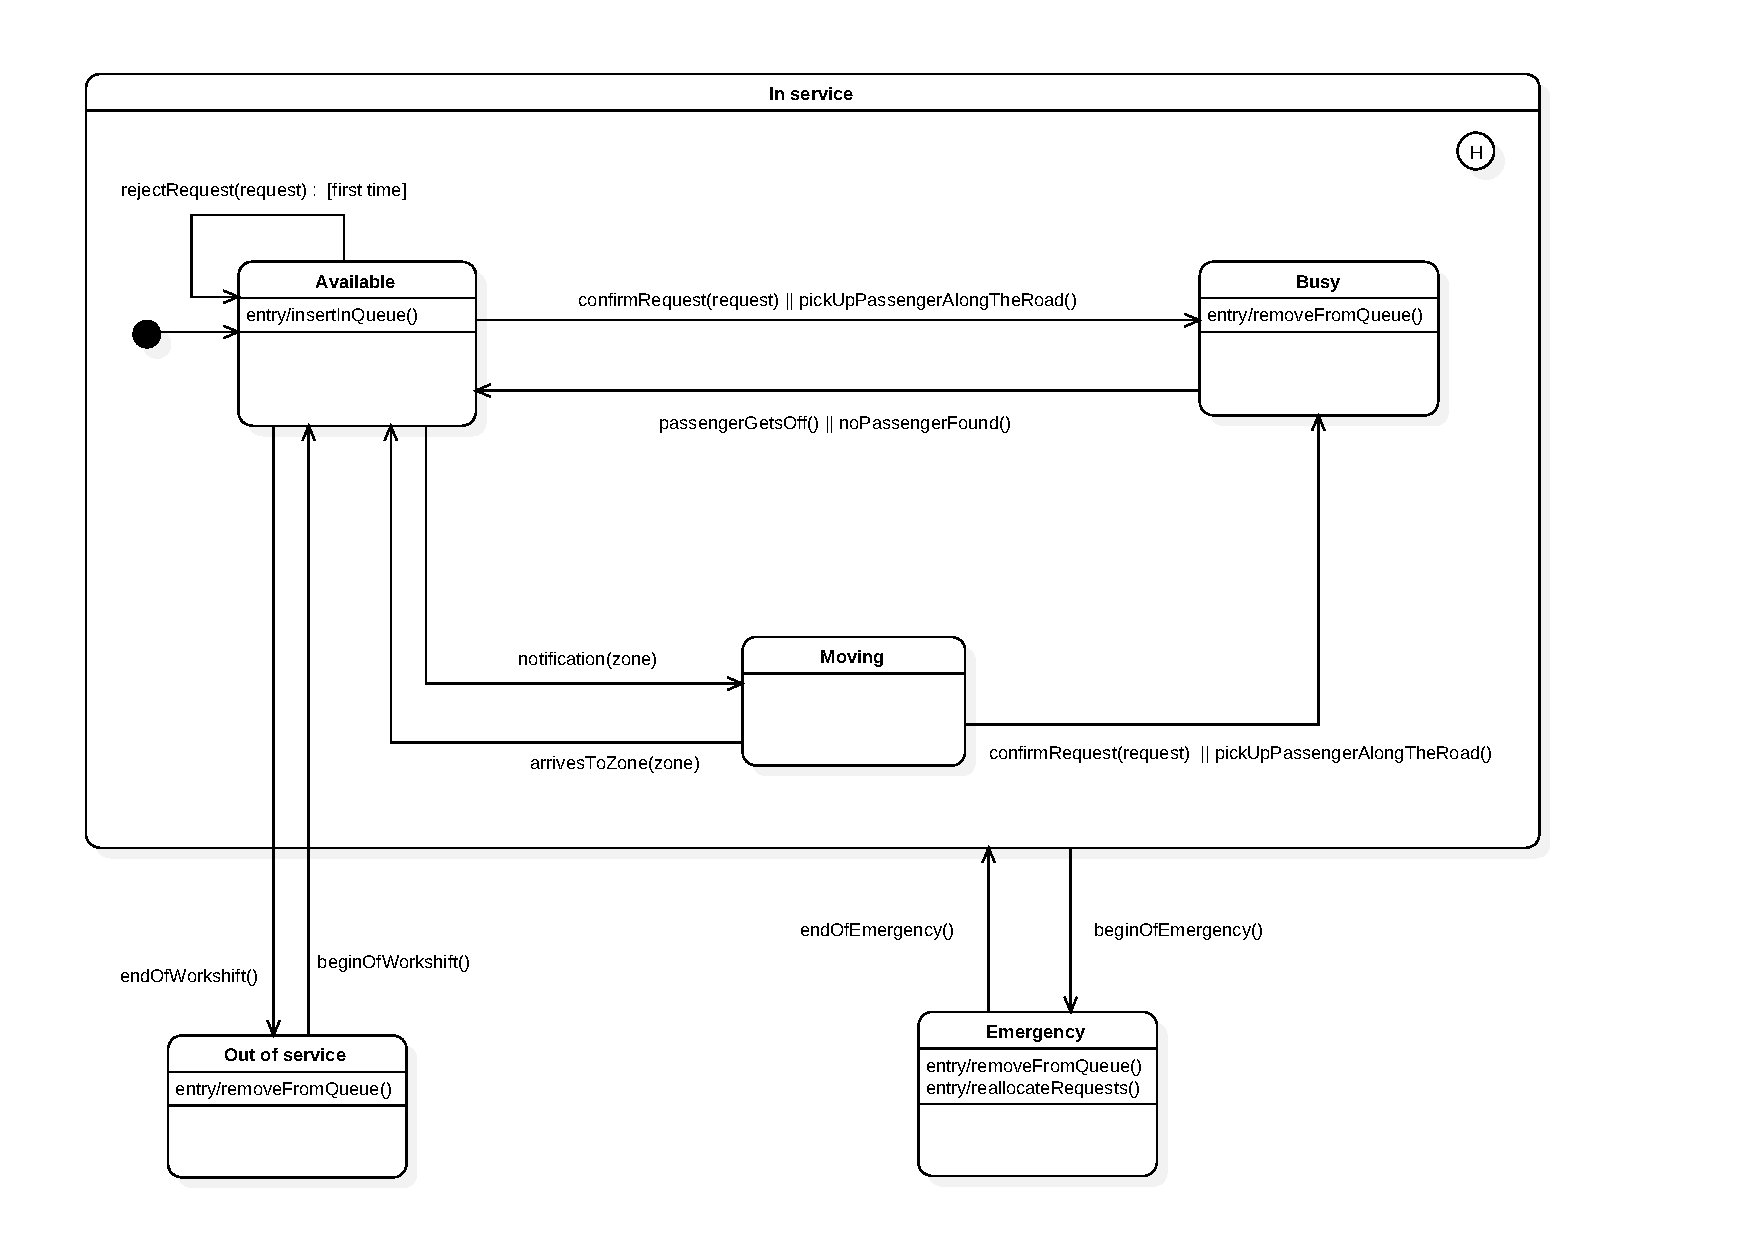
\includegraphics[bb=20bp 20bp 800bp 575bp,scale=0.6]{specific-requirements/3.6-other-uml/image/state}
\par\end{centering}

\protect\caption{Taxi state - UML State Chart diagram }


\end{figure}


\end{landscape}

\clearpage{}


\subsubsection{Activity diagram}

Since in the previous section for the request evaluation only a normal
flow has been represented, here we show an activity diagram in order
to clarify how the general flow (normal flow and exceptional flow)
of that use case works.

\begin{figure}[H]
\begin{centering}
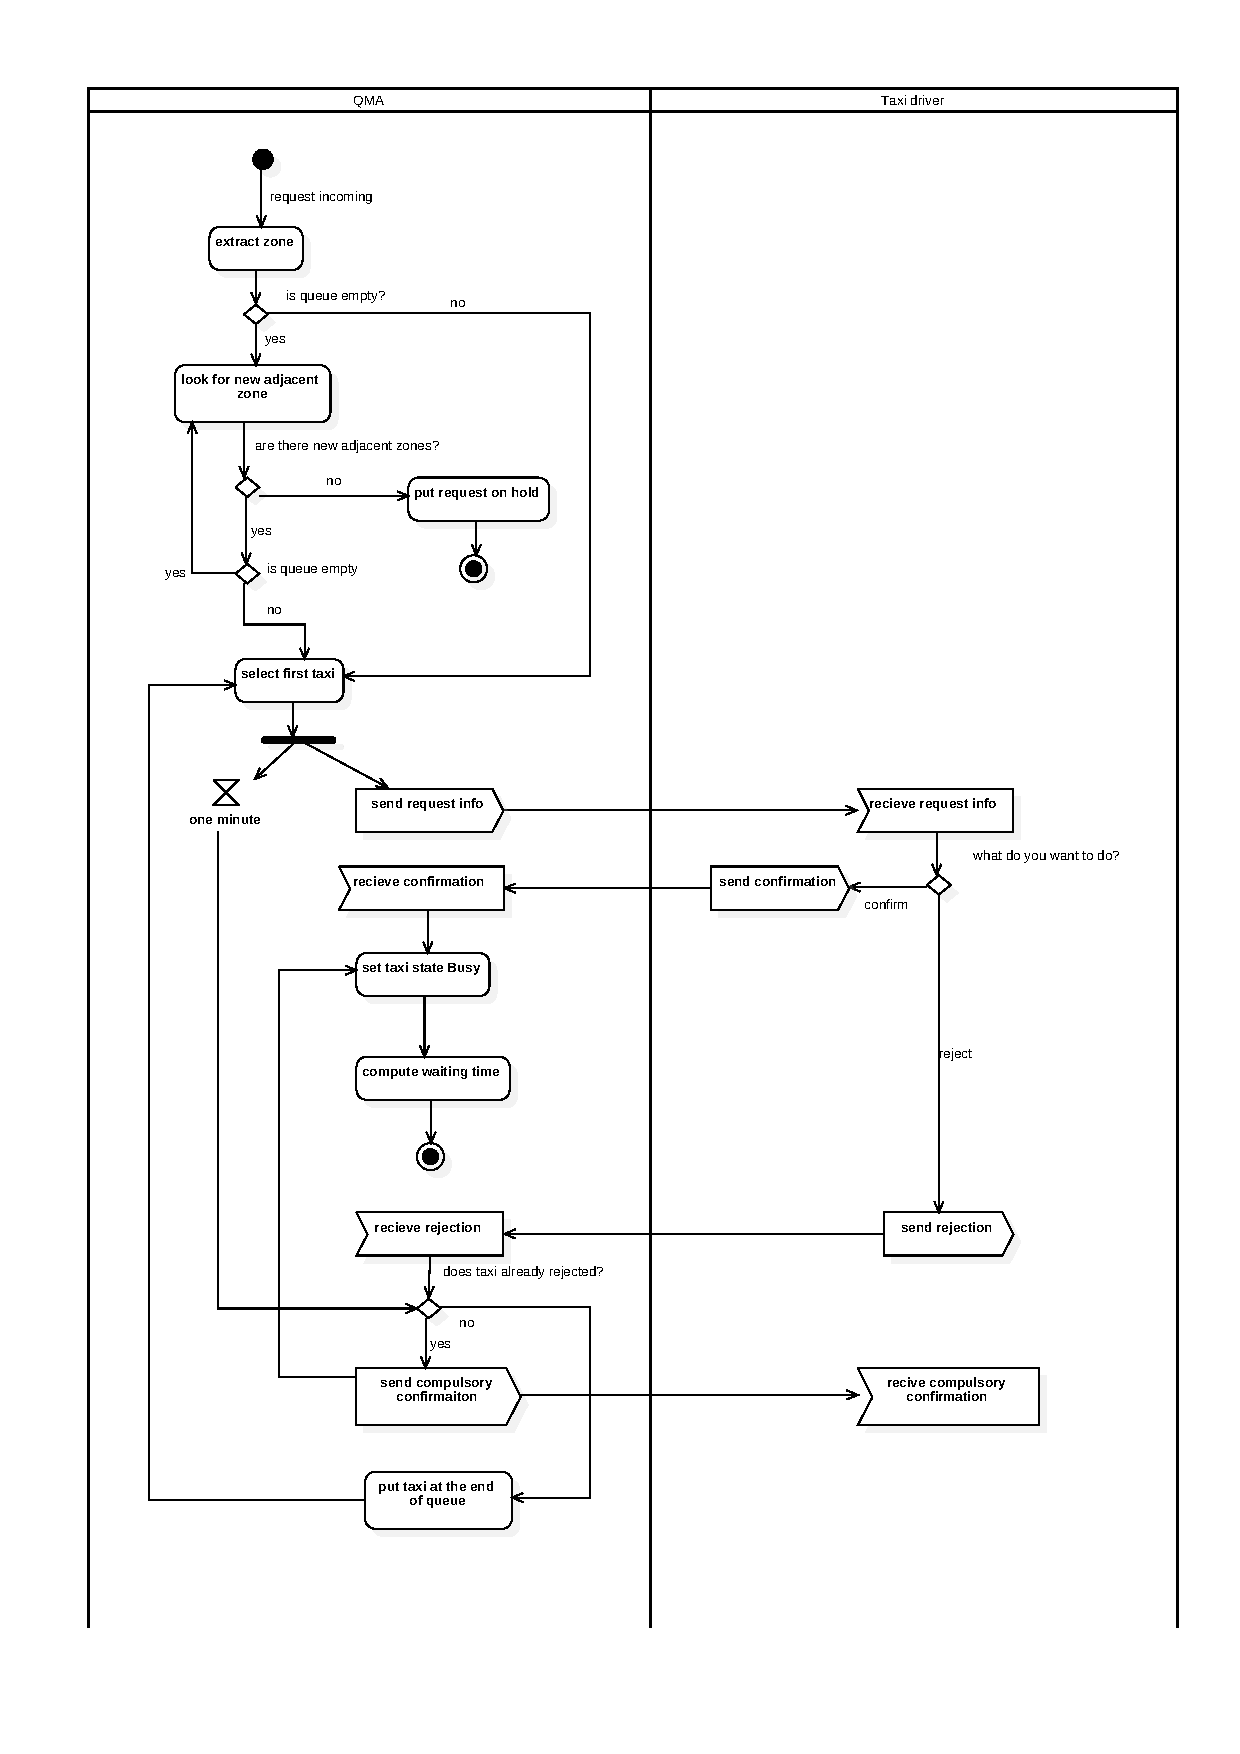
\includegraphics[bb=20bp 60bp 580bp 815bp,scale=0.7]{specific-requirements/3.6-other-uml/image/activity}
\par\end{centering}

\protect\caption{Request evaluation - UML Activity diagram}


\end{figure}

